%\documentclass[10pt]{beamer}
\documentclass[handout,10pt]{beamer}
%\usepackage{xeCJK}

%\usepackage[orientation=landscape,size=custom,width=16,height=12,scale=0.5,debug]{beamerposter}

 % 1. packages

 % ----------- fonts and symbles ---------
\usepackage{amsmath,amssymb,amsfonts,amsthm}
%\usepackage{CJK}
\usepackage{dsfont}
\usepackage{mathrsfs}
\usepackage{eucal} % for \mathcal

%\renewcommand{\rmdefault}{ptm}


%\usepackage{fontspec}
%\newfontfamily\monaco{Monaco}

%\usepackage{mathbbold} %,bbold

 \usepackage{textcomp} % for \textnormal{\textperthousand}
% -----------------





%\usepackage{slashbox}
%\usepackage[margin=2.2cm]{geometry} % |geometry| package clash with |booktabs| package
%\usepackage{cases}
% -------- tables -------
\usepackage{booktabs} % for \toprule, \bottomrule
\usepackage{tabularx}
\usepackage{multirow}
% --------- figures ---------
\usepackage{graphicx}
% ---------- algorithms -------
\usepackage{algorithm}
\usepackage{algorithmic}
%\usepackage{footnote}
    % |footnote| package occurs error:
    % Runaway argument?
    % \def \insertfootnotetext {\@@ }\def \insertfootnotemark {\@makefnmark \ETC.

\usepackage{listings}

\usepackage[linewidth=1pt]{mdframed} % for  mdframe environment




 \usepackage{color}
 \usepackage{xcolor}     %¸ßÁÁʹÓõÄÑÕÉ«

\usepackage{setspace}
%%\usepackage{type1cm}
\usepackage{adjustbox} % for \adjustbox

\usepackage{accsupp}
\newcommand{\emptyaccsupp}[1]{\BeginAccSupp{ActualText={}}#1\EndAccSupp{}}




%%   figures and tables
\graphicspath{{figure/}}


% 2. new commands

% 2.0 common commands
%\newcommand{\bc}{\begin{center}}
%\newcommand{\ec}{\end{center}}
%\newcommand{\ba}{\begin{array}}
%\newcommand{\ea}{\end{array}}
%\newcommand{\be}{\begin{equation}}
%\newcommand{\ee}{\end{equation}}

% 2.1 colors
\definecolor{dgrey}{rgb}{0.30,0.30,0.30}
\definecolor{lred}{rgb}{0.50,0.00,0.50}
\definecolor{lblue}{rgb}{0.8,0.8,1}
\definecolor{dred}{rgb}{0.6,0,0}
\definecolor{dblue}{rgb}{0,0,0.5}
\definecolor{dgrey}{rgb}{0.35,0.35,0.35}
\definecolor{rred}{rgb}{0.9,0,0}
\definecolor{mylblue}{rgb}{0.3,0.2, 0.8}

\definecolor{commentcolor}{RGB}{85,139,78}
\definecolor{stringcolor}{RGB}{206,145,108}
\definecolor{keywordcolor}{RGB}{34,34,250}
\definecolor{backcolor}{RGB}{220,220,220}

\newcommand{\blue}[1]{{\color{blue}#1}}
\newcommand{\dblue}[1]{{\color{dblue}#1} }
\newcommand{\red}[1]{{\color{red}#1}}
\newcommand{\dred}[1]{{\color{dred}#1}}
\newcommand{\cyan}[1]{{\color{cyan}#1}}
\newcommand{\bfblue}[1]{\textbf{\color{dblue}#1} }
\newcommand{\bfred}[1]{\textbf{\color{dred}#1} }
\newcommand{\green}[1]{{\color{green}#1}}
%\newcommand{\alert}[1]{{\color{red}#1}}
\newcommand{\black}[1]{{\color{black}#1}}
\newcommand{\light}[1]{{\color{blue}\textbf{#1}}}
\newcommand{\hot}[1]{{\color{dred}#1}}
 \newcommand{\highlight}[1]{ \textbf{\color{mylblue}#1}}
 \newcommand{\important}[1]{{\color{red}#1}} % for highlighting  some words

 \newcommand{\mystar}{\dred{$^{\clubsuit}$ }}
  \newcommand{\doublestar}{\dred{$^{\clubsuit\clubsuit}$ }}

\newcommand{\mynote}[1]{{\footnotesize \color{mylblue}#1}}

 \newcommand{\hint}[1]{{\small \color{mylblue}#1}}
\newcommand{\smallhint}[1]{{\small \color{dgrey}#1}}
\newcommand{\footnotehint}[1]{{\footnotesize \color{dgrey}#1}}
\newcommand{\tinyhint}[1]{{\tiny \color{dgrey}#1}}
\newcommand{\mytitle}[1]{\medskip{\large \textbf{\color{mylblue}#1}}}
\newcommand{\normaltitle}[1]{\medskip{ \textbf{\color{mylblue}#1}}}

%\newcommand{\head}[1]{\textbf{\large\color{blue}#1}}
%\newcommand{\heading}[1]{\textbf{\large\color{blue}#1}}

\newcommand{\myfbox}[2]{ \bigskip \begin{center} \fbox{\parbox{#1}{ #2  }} \end{center}\bigskip }

\newcommand{\myvar}[1]{}
%\newcommand{\mynote}[1]{#1}

% 2.2 mathematical symbols

\newcommand{\drightarrow}{\stackrel{d.}{\rightarrow}}
\newcommand{\prightarrow}{\stackrel{p.}{\rightarrow}}
\newcommand{\bernoulli}{\textnormal{Ber}}
\newcommand{\cov}{\mathsf{Cov}}
\newcommand{\corr}{\mathbf{Corr}}
\newcommand{\regret}{\textnormal{Regret}}
\newcommand{\conv}{\textnormal{conv}}
\newcommand{\dotdiv}{\stackrel{\centerdot}{-}}
\newcommand{\dom}{\textnormal{dom}}
\newcommand{\convergenceinprob}{\stackrel{P}{\rightarrow}}
\newcommand{\convergenceindist}{\rightsquigarrow}
\newcommand{\probability}{\mathbb{P}}
\newcommand{\expectation}{\mathbb{E}}
\newcommand{\epi}{\textnormal{epi}}
\newcommand{\variance}{\mathbb{V}}
\newcommand{\var}[1]{\mathbb{V}(#1)}
\newcommand{\covariance}{\mathsf{Cov}}
\newcommand{\empiricalrisk}[1]{\hat{R}(#1)}
\newcommand{\expectedrisk}[1]{R(#1)}
\newcommand{\mgf}[1]{\psi_{#1}(\lambda)}
\newcommand{\mgfexpansion}[1]{\expectation[e^{\lambda#1}]}
\newcommand{\mgfmultivariate}[1]{\expectation[e^{\lambda^\transpose#1}]}
\newcommand{\transpose}{{\mathsf{T}}}
\newcommand{\real}{\mathbb{R}}
\newcommand{\gaussian}[2]{\mathcal{N}(#1,#2)}
\newcommand{\subGaussian}[1]{\mathsf{subG}(#1)}
\newcommand{\indicator}[1]{\mathbb{I}[#1]}
\newcommand{\x}[1]{x^{(#1)}}
\newcommand{\y}[1]{y^{(#1)}}
\newcommand{\z}[1]{z^{(#1)}}
\newcommand{\feature}{x}
\newcommand{\response}{y}
\newcommand{\supofempiricalprocess}{\|\mathbb{P}_n-\mathbb{P}\|_{\decisionspace}}
\newcommand{\decisionspace}{\mathscr{F}}
\newcommand{\decisionfunction}{f}
\newcommand{\featurespace}{\mathcal{X}}
\newcommand{\classifierestimate}{\widehat{h}}
\newcommand{\classifiertrue}{h^\star}
\newcommand{\classifier}{h}
\newcommand{\hypothesisclass}{\mathcal{H}}
\newcommand{\dataset}{\mathcal{D}}
\newcommand{\defineas}{\stackrel{\textnormal{def}}{=}}
\newcommand{\rademachercomplexity}[1]{\mathsf{Rad}_n\left(#1\right)}
\newcommand{\loss}{\ell}
\newcommand{\composite}{\circ}
\newcommand{\convexhull}{\mathsf{conv}}
\newcommand{\norm}[2][2]{\|#2\|_{#1}}
\newcommand{\shatteringcoefficient}[2]{\mathcal{S}(#1,#2)}
\newcommand{\vcdimension}[1]{\mathsf{VC}\left(#1\right)}
\newcommand{\rank}{\mathsf{rank}}
\newcommand{\innerproduct}[2]{\left\langle #1, #2\right\rangle}
\newcommand{\modelparameter}{\theta}
\newcommand{\ball}[3][]{\mathcal{B}_{{#1}}\left(#2,#3\right)}
\newcommand{\metric}{d}
\newcommand{\coveringnumber}[4][]{N_{{#1}}\left(#2,#3,#4\right)}
\newcommand{\trace}{\textnormal{tr}}
\newcommand{\std}{\textnormal{std}}
\newcommand{\sgn}{\textnormal{sign}}
%\renewcommand{\span}{\textnormal{span}}

 % do not overwrite the existing command \span
 % as it leads to an error of
 %  "Missing # Inserted in Alignment Preamble" for ``align'' environment

\newcommand{\myspan}{\textnormal{span}}

%%%
\newcommand{\rightarrowd}{\stackrel{d}{\rightarrow}}
\newcommand{\rightarrowp}{\stackrel{p}{\rightarrow}}
\newcommand{\defeq}{ \stackrel{\textnormal{def}}{=}}
\newcommand{\proj}{ \textnormal{Proj}}
\newcommand{\dist}{\textnormal{dist}}

\newcommand{\argmax}{\textnormal{argmax}}
\newcommand{\argmin}{\textnormal{argmin}}
\newcommand{\subg}{\textnormal{subG}}


 \newcommand{\bba}{\mathbb{A}}
\newcommand{\bbb}{\mathbb{B}}
\newcommand{\bbc}{\mathbb{C}}
\newcommand{\bbd}{\mathbb{D}}
\newcommand{\bbe}{\mathbb{E}}
\newcommand{\bbf}{\mathbb{F}}
\newcommand{\bbg}{\mathbb{G}}
\newcommand{\bbh}{\mathbb{H}}
\newcommand{\bbi}{\mathbb{I}}
\newcommand{\bbj}{\mathbb{J}}
\newcommand{\bbk}{\mathbb{K}}
\newcommand{\bbl}{\mathbb{L}}
\newcommand{\bbm}{\mathbb{M}}
\newcommand{\bbn}{\mathbb{N}}
\newcommand{\bbo}{\mathbb{O}}
\newcommand{\bbp}{\mathbb{P}}
\newcommand{\bbq}{\mathbb{Q}}
\newcommand{\bbr}{\mathbb{R}}
\newcommand{\bbs}{\mathbb{S}}
\newcommand{\bbt}{\mathbb{T}}
\newcommand{\bbu}{\mathbb{U}}
\newcommand{\bbv}{\mathbb{V}}
\newcommand{\bbw}{\mathbb{W}}
\newcommand{\bbx}{\mathbb{X}}
\newcommand{\bby}{\mathbb{Y}}
\newcommand{\bbz}{\mathbb{Z}}

\newcommand{\bfa}{\mathbf{a}}
\newcommand{\bfb}{\mathbf{b}}
\newcommand{\bfc}{\mathbf{c}}
\newcommand{\bfd}{\mathbf{d}}
\newcommand{\bfe}{\mathbf{e}}
\newcommand{\bff}{\mathbf{f}}
\newcommand{\bfg}{\mathbf{g}}
\newcommand{\bfh}{\mathbf{h}}
\newcommand{\bfi}{\mathbf{i}}
\newcommand{\bfj}{\mathbf{j}}
\newcommand{\bfk}{\mathbf{k}}
\newcommand{\bfl}{\mathbf{l}}
\newcommand{\bfm}{\mathbf{m}}
\newcommand{\bfn}{\mathbf{n}}
\newcommand{\bfo}{\mathbf{o}}
\newcommand{\bfp}{\mathbf{p}}
\newcommand{\bfq}{\mathbf{q}}
\newcommand{\bfr}{\mathbf{r}}
\newcommand{\bfs}{\mathbf{s}}
\newcommand{\bft}{\mathbf{t}}
\newcommand{\bfu}{\mathbf{u}}
\newcommand{\bfv}{\mathbf{v}}
\newcommand{\bfw}{\mathbf{w}}
\newcommand{\bfx}{\mathbf{x}}
\newcommand{\bfy}{\mathbf{y}}
\newcommand{\bfz}{\mathbf{z}}

\newcommand{\bfA}{\mathbf{A}}
\newcommand{\bfB}{\mathbf{B}}
\newcommand{\bfC}{\mathbf{C}}
\newcommand{\bfD}{\mathbf{D}}
\newcommand{\bfE}{\mathbf{E}}
\newcommand{\bfF}{\mathbf{F}}
\newcommand{\bfG}{\mathbf{G}}
\newcommand{\bfH}{\mathbf{H}}
\newcommand{\bfI}{\mathbf{I}}
\newcommand{\bfJ}{\mathbf{J}}
\newcommand{\bfK}{\mathbf{K}}
\newcommand{\bfL}{\mathbf{L}}
\newcommand{\bfM}{\mathbf{M}}
\newcommand{\bfN}{\mathbf{N}}
\newcommand{\bfO}{\mathbf{O}}
\newcommand{\bfP}{\mathbf{P}}
\newcommand{\bfQ}{\mathbf{Q}}
\newcommand{\bfR}{\mathbf{R}}
\newcommand{\bfS}{\mathbf{S}}
\newcommand{\bfT}{\mathbf{T}}
\newcommand{\bfU}{\mathbf{U}}
\newcommand{\bfV}{\mathbf{V}}
\newcommand{\bfW}{\mathbf{W}}
\newcommand{\bfX}{\mathbf{X}}
\newcommand{\bfY}{\mathbf{Y}}
\newcommand{\bfZ}{\mathbf{Z}}


\newcommand{\bfSigma}{\mathbf{\Sigma}}
\newcommand{\bfrho}{\mathbf{\rho}}

\newcommand{\cala}{\mathcal{A}}
\newcommand{\calb}{\mathcal{B}}
\newcommand{\calc}{\mathcal{C}}
\newcommand{\cald}{\mathcal{D}}
\newcommand{\cale}{\mathcal{E}}
\newcommand{\calf}{\mathcal{F}}
\newcommand{\calg}{\mathcal{G}}
\newcommand{\calh}{\mathcal{H}}
\newcommand{\cali}{\mathcal{I}}
\newcommand{\calj}{\mathcal{J}}
\newcommand{\calk}{\mathcal{K}}
\newcommand{\call}{\mathcal{L}}
\newcommand{\calm}{\mathcal{M}}
\newcommand{\caln}{\mathcal{N}}
\newcommand{\calo}{\mathcal{O}}
\newcommand{\calp}{\mathcal{P}}
\newcommand{\calq}{\mathcal{Q}}
\newcommand{\calr}{\mathcal{R}}
\newcommand{\cals}{\mathcal{S}}
\newcommand{\calt}{\mathcal{T}}
\newcommand{\calu}{\mathcal{U}}
\newcommand{\calv}{\mathcal{V}}
\newcommand{\calw}{\mathcal{W}}
\newcommand{\calx}{\mathcal{X}}
\newcommand{\caly}{\mathcal{Y}}
\newcommand{\calz}{\mathcal{Z}}


% 3. theorem and environments

%\newtheorem{theorem}{Theorem}%[section]
\newtheorem{proposition}{Proposition}%[section]
%\newtheorem{property}{Property}%[section]
%\newtheorem{lemma}{Lemma}%[section]
%\newtheorem{corollary}{Corollary}%[section]
%\newtheorem{definition}{Definition}%[section]
%\newtheorem{example}{Example}%[section]
%\newtheorem{remark}{Remark}%[section]
%\newtheorem{note}{Note}%[section]
%\newtheorem{problem}{Problem}%[section]
\newtheorem{exercise}{Exercise}
%\newtheorem{assumption}{Assumption}
\newtheorem*{lemma_star}{Lemma}
\newtheorem*{theorem_star}{Theorem}

%\newenvironment{summary}[1][Summary]{\par\medskip   \color{dred}\textbf{\large#1. } }{ \medskip}
%\newenvironment{remark}[1][Remark]{\par\medskip  \begin{small} \color{dblue}\textbf{#1. } }{ \end{small}\medskip}
%\renewenvironment{proof}[1][Proof]{\noindent\textbf{#1.} }{\mbox{} \hfill{\small\textrm{$\Box$}}\vspace{1ex}}
% \newenvironment{answer}[1][Answer]{\par\medskip \color{dblue}\textbf{\large#1. }}{ \medskip}

\newenvironment{summary}[1][总结]{\par\medskip   \color{dred}\textbf{\large#1 } }{ \medskip}
\newenvironment{remark}[1][注意]{\par\medskip   \color{dblue}\textbf{\large#1 } }{ \medskip}
\newenvironment{footnoteremark}{ \color{dblue}\begin{footnotesize} }{\end{footnotesize}}
\renewenvironment{proof}[1][证明]{\noindent\textbf{#1.} }{\mbox{} \hfill{\small\textrm{$\Box$}}\vspace{1ex}}
 \newenvironment{question}[1][Q.]{\par\medskip {\color{lred}\large#1}}{ \medskip}
 \newenvironment{answer}[1][Answer]{\par\medskip \color{dblue}\textbf{\large#1 }}{ \medskip}

% 4. beamer setting




%\newtheorem{definition}{\textbf{¶¨Òå}}[section]
%\newtheorem{proposition}[definition] { \textbf{ÃüÌâ}}
%\newtheorem{lemma}[definition] { \textbf{ÒýÀí}}
%\newtheorem{theorem}[definition]{ \textbf{¶¨Àí}}
%\newtheorem{corollary}[definition] { \textbf{ÍÆÂÛ}}
%\newtheorem{remark}[definition] { \textbf{×¢}}
%\newtheorem{example}[definition] { \textbf{Àý}}

%\newcommand{\shadow}[1]{\begin{center}
%\bf{\textcolor{dblue}{\shadowbox{\parbox{3.8in}
% {\textcolor{red}
% {\vspace{1mm}#1}}}}}
%\end{center}}
%
%\newcommand{\head}[1]{\begin{center}
%\bf{\textcolor{dblue}{\shadowbox{\parbox{3.8in}
% {\textcolor{dred}
% {\vspace{1mm}#1}}}}}
%\end{center}}
%
%
%\newcommand{\heading}[1]{%
%  \begin{center}
%    \large\bf
%    \shadowbox{#1}%
%  \end{center}
%\vspace{1ex minus 1ex}}

% set  space above and below math equations in display style

\expandafter\def\expandafter\normalsize\expandafter{%
    \normalsize
    \setlength\abovedisplayskip{1.5ex}
    \setlength\belowdisplayskip{1.2ex}
    \setlength\abovedisplayshortskip{0.5ex}
    \setlength\belowdisplayshortskip{0.5ex}
}

% Ìí¼ÓÒ³Âë´úÂ룬¹È¸èÕÒµ½µÄ¡£
\addtobeamertemplate{navigation symbols}{}{%
    %\usebeamerfont{footline}%
    %\usebeamercolor[fg]{footline}%
    \setbeamercolor{footline}{fg=blue}
    \setbeamerfont{footline}{series=\bfseries}
    \hspace{1em}%
    \normalsize{\insertframenumber/\inserttotalframenumber}
}

% section numbering
\setbeamertemplate{section in toc}[sections numbered]
\setbeamertemplate{subsection in toc}[subsections numbered]



\lstset{                        %¸ßÁÁ´úÂëÉèÖÃ
%basicstyle=\small, % print whole listing small
%basicstyle=\footnotesize\sffamily, % print whole listing small
basicstyle=\footnotesize\rmfamily, % print whole listing small
%basicstyle=\rmfamily, % print whole listing small
    language=python,                    %PythonÓï·¨¸ßÁÁ
    %linewidth=0.9\linewidth,            %Áбílist¿í¶È
    %basicstyle=\ttfamily,              %ttÎÞ·¨ÏÔʾ¿Õ¸ñ
    commentstyle=\color{commentcolor},  %×¢ÊÍÑÕÉ«
    keywordstyle=\color{keywordcolor},  %¹Ø¼ü´ÊÑÕÉ«
    stringstyle=\color{stringcolor},    %×Ö·û´®ÑÕÉ«
    %showspaces=true,                   %ÏÔʾ¿Õ¸ñ
    numbers=left,                       %ÐÐÊýÏÔʾÔÚ×ó²à
    %numberstyle=\tiny\emptyaccsupp,     %ÐÐÊýÊý×Ö¸ñʽ
    numberstyle=\tiny,                  %ÐÐÊýÊý×Ö¸ñʽ
    numbersep=5pt,                      %Êý×Ö¼ä¸ô
    frame=single,                       %¼Ó¿ò
    framerule=0pt,                      %²»»®Ïß
    %escapeinside=@@,                    %ÌÓÒݱêÖ¾
    escapeinside=``,                    %ÌÓÒݱêÖ¾
    emptylines=1,                       %
    xleftmargin=3em,                    %list×ó±ß¾à
    backgroundcolor=\color{backcolor},  %ÁÐ±í±³¾°É«
    tabsize=4,                          %ÖƱí·û³¤¶ÈΪ4¸ö×Ö·û
    %gobble=4                            %ºöÂÔÿÐдúÂëÇ°4¸ö×Ö·û
    breaklines=true,
    extendedchars=false
    }

\lstdefinestyle{numbers}{numbers=left, stepnumber=1, numberstyle=\tiny, numbersep=10pt}
 \lstdefinestyle{nonumbers}{numbers=none}

\newcommand{\alertcode}[1]{{\color{red}#1}} % used for alerting codes

%\lstset{numbers=left, numberstyle=\tiny,
%keywordstyle=\color{blue!70},
%commentstyle=\color{red!50!green!50!blue!50},
%frame=shadowbox,
%rulesepcolor=\color{red!20!green!20!blue!20},
%escapeinside=``,
%framesep = 2ex,
%rulesep = 1ex
%%framexrightmargin= 1em %
%}


% Vary the color applet  (try out your own if you like)
\colorlet{structure}{red!65!black}

%\beamertemplateshadingbackground{yellow!50}{white}


%\setbeamerfont{normal text}{family=\rmfamily}
%\setbeamerfont{frametitle}{family=\rmfamily}

% Changing the fonts: this will make the slides more readable and the math look like regular tex math
\usefonttheme{serif}



% set spaces

\setstretch{1.2}  % ÉèÖÃÐоà

\addtobeamertemplate{block begin}{\setlength\abovedisplayskip{0pt}} % reduce the large space before a block

% set section number styles



\newcommand{\secno}{Sec.\,\thesection\ }
\newcommand{\subsecno}{Sec.\,\thesubsection\ }

% set logo

 \pgfdeclareimage[width=1.0]{small-logo}{SMaLL.jpg}
%
 \logo{\vbox{\vskip0.1 \hbox{\pgfuseimage{small-logo}}}}

% set math equation fontsize

 \makeatletter
\DeclareMathSizes{\f@size}{10}{5}{5}
\makeatother

% for chinese section name
\hypersetup{CJKbookmarks=true}

\usepackage{ctex}

%\usepackage{hyperref}
%\hypersetup{hidelinks,
%	colorlinks=true,
%	allcolors=black,
%	pdfstartview=Fit,
%	breaklinks=true}
	
\begin{document}
\hypersetup{CJKbookmarks=true}
	
\addtobeamertemplate{block begin}{\setlength\abovedisplayskip{0pt}}

\setbeamertemplate{itemize items}{\color{black}$\bullet$}
	
\title[数值优化]{第二章 凸函数}
	
\bigskip
	
\author[]{
	\underline{SMaLL}
}

\institute[CUP]{
	\inst{1}
	中国石油大学(华东)\\
	SMaLL 课题组: 梁锡军  \\
	\blue{small.sem.upc.edu.cn}\\
	liangxijunsd@163.com \\ 
}

\date[2023]{\small    2023}
% set logo
\pgfdeclareimage[ width=1.0cm]{small-logo}{SMaLL}
%
\logo{\vbox{\vskip0.1cm\hbox{\pgfuseimage{small-logo}}}}

		
		
\subject{ optimization}
	
\frame{\titlepage}
	


\frame{
    \frametitle{第2章 凸函数\quad (Convex Functions)}
    \tableofcontents[hideallsubsections]% 显示在目录中加亮的当前章节
  }

%%
%% 定义框架页
%%
\AtBeginSection[]{       % 在每个Section 前都会加入的Frame
  %\frame<handout:1>{
  \begin{frame}
    \frametitle{第2章 凸函数\quad (Convex Functions)}
    %\tableofcontents[current,currentsubsection] % 显示在目录中加亮的当前章节
    %\tableofcontents[hideallsubsections,currentsection] % 显示在目录中加亮的当前章节
    \tableofcontents[current,hideallsubsections]
  \end{frame}

  %}
}



\section{基本性质和示例}
\begin{frame}
\mytitle{\secno \secname}

\normaltitle{定义}
	$f: \mathbb{R}^{n} \rightarrow \mathbb{R}$ 是凸函数, 如果$\textbf{dom} \ f$ 是凸集,且
    \begin{equation}
	f(\theta x+(1-\theta) y) \leq \theta f(x)+(1-\theta) f(y)
    \end{equation}
任意 $x, y \in \textbf{dom}\  f, 0 \leq \theta \leq 1$
\footnotehint{\quad $\dom f  = \{x\in \bbr^n: f(x)<\infty\}$}
    \begin{figure}[htbp]
    \centering
   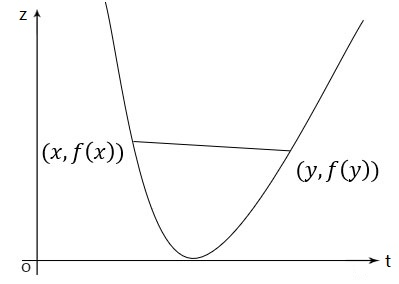
\includegraphics[height=3cm,width=5cm]{修改_第二章图2-1}
    %\caption{Definition}
    \end{figure}
    \begin{itemize}
    	\item 如果$-f$ 是凸函数,那么$f$ 是凹函数 
    	\item 如果 $\textbf{dom} \ f$ 是凸的并且满足以下式子,那么$f$ 是严格凸的
    	\begin{equation}
    		f(\theta x+(1-\theta) y)<\theta f(x)+(1-\theta) f(y)
    	\end{equation}
    	任意 $x, y \in \textbf{dom}\ f, x \neq y, 0<\theta<1$
    \end{itemize}
\end{frame}

\begin{frame}
  \frametitle{讨论}

  \vspace{5ex}
  \normaltitle{Q. 你知道哪些函数是凸函数或凹函数? }
\end{frame}

%------------------------------------------
\begin{frame}
	\frametitle{在 $\bbr$上的示例}
	凸函数:
	\begin{itemize}
		\item 仿射函数: $a x+b$ 在$\mathbb{R}上,$ 任意 $a, b \in \mathbb{R}$
		\item 指数函数: $e^{a x},$ 任意 $a \in \mathbb{R}$
		\item 幂函数: $x^{\alpha}$ on $\mathbb{R}_{++},$ 当 $\alpha \geq 1$ 或 $\alpha \leq 0$时
		\item 绝对值幂函数: $|x|^{p}$ 在 $\mathbb{R}上,$ 当 $p \geq 1$时
		\item 负熵函数: $x \log x$ 定义域为 $\mathbb{R}_{++}$

	\end{itemize}
    \bigskip
    \bigskip
    凹函数:
    \begin{itemize}
    	\item 仿射函数: $a x+b$ 在$\mathbb{R}上,$ 任意$a, b \in \mathbb{R}$
    	\item 幂函数: $x^{\alpha}$ 在 $\mathbb{R}_{++}上,$ 当 $0 \leq \alpha \leq 1$时
    	\item 对数函数: $\log x$ 在 $\mathbb{R}_{++}$上
    \end{itemize}
\end{frame}
%-------------------------------------------
\begin{frame}
\frametitle{在$\mathbb{R}^n$ 和 $\mathbb{R}^{m\times n}$上的示例}

	* 仿射函数是凸的也是凹的;

\dred{    * 所有范数都是凸的 }

\onslide<2->{
    \textbf{在$\mathbb{R}^{n}$上的示例}
    \begin{itemize}
    	\item 仿射函数 $f(x)=a^{T} x+b$
    	\item 范数: $\|x\|_{p}=\left(\sum_{i=1}^{n}\left|x_{i}\right|^{p}\right)^{1 / p}$, $p \geq 1$; 
    	
    	$\|x\|_{\infty}=\max _{k}\left|x_{k}\right|$
    \end{itemize}
}

  \onslide<3->{
    \bigskip
    \textbf{在$\ \mathbb{R}^{m \times n}(m \times n$矩阵)上的示例}
    \begin{itemize}
    	\item 仿射函数
    	\begin{equation}
    		f(X)=\textbf{tr}\left(A^{T} X\right)+b=\sum_{i=1}^{m} \sum_{j=1}^{n} A_{i j} X_{i j}+b
    	\end{equation}
    	\item 谱(最大奇异值)范数
    	\begin{equation}
    		f(X)=\|X\|_{2}=\sigma_{\max }(X)=\left(\lambda_{\max }\left(X^{T} X\right)\right)^{1 / 2}
    	\end{equation}
    \end{itemize}
 }

\end{frame}

%----------------------------------------------
\begin{frame}
	\frametitle{扩展值扩展}
	
$f$的扩展值扩展 $\tilde{f}$ 是
	\begin{equation}
	\tilde{f}(x)=f(x), \quad x \in \textbf{dom}\  f, \quad \tilde{f}(x)=\infty, \quad x \notin \textbf{dom}\ f
	\end{equation}
    经常简化记法;


    % for example, the condition

\onslide<2->{
%\begin{示例}
\hint{示例:}
  [凸集的指示函数]
  \begin{equation}
    I_C(x) = \left\{
    \begin{array}{cl}
        0, & x\in C\\
        \infty,  & x\not\in C. \\
    \end{array}
    \right.
  \end{equation}
%\end{example}
}
\end{frame}


\begin{frame}
	\frametitle{凸函数限制在直线上}

\begin{mytheorem}
	$f: \mathbb{R}^{n} \rightarrow \mathbb{R}$ 是凸函数 $\Leftrightarrow$
   函数 $g: \mathbb{R} \rightarrow \mathbb{R}$
	\begin{equation}
		g(t)=f(x+t v), \quad \textbf{dom}\ g=\{t \mid x+t v \in \textbf{dom}\ f\}
	\end{equation}
    是在$t$上的凸函数 ,对于任意 $x \in \textbf{dom} f, v \in \mathbb{R}^{n}$
 \end{mytheorem}
    %can check convexity of $f$ by checking convexity of functions of one variable\\
    %\bigskip

    \onslide<2->{
   \begin{myexample} $f: \mathbf{S}^{n} \rightarrow \mathbb{R}$ with $\hint{f(X)=\log \text{det} X,} \textbf{dom} f=\mathbf{S}_{++}^{n}$
    \begin{equation}
    	\begin{aligned}
        g(t)=\log \text{det}(X+t V) &=\log \text{det} X+\log \text{det}\left(I+t X^{-1 / 2} V X^{-1 / 2}\right) \\
        &=\log \text{det} X+\sum_{i=1}^{n} \log \left(1+t \lambda_{i}\right)
        \end{aligned}
    \end{equation}
    其中 $\lambda_{i}$ 是 $X^{-1 / 2} V X^{-1 / 2}$的特征值\\
    \bigskip
    $g$ 在 $t$上是凹的 (对于任意 $X \succ 0, V)$; $\Rightarrow$ $f$ 是凹的
    \end{myexample}
    \hint{Ex. }
    }
\end{frame}

%-------------------------------------------
\begin{frame}
	\frametitle{一阶条件}
	$f$ 是 \textbf{可微分的} ,即它的梯度
	\begin{equation}
		\nabla f(x)=\left(\frac{\partial f(x)}{\partial x_{1}}, \frac{\partial f(x)}{\partial x_{2}}, \ldots, \frac{\partial f(x)}{\partial x_{n}}\right)
	\end{equation}
    在每个 $x \in \textbf{dom} f$上存在,$\textbf{dom} f$ 是开放的


    \begin{mytheorem}
      [一阶条件**] 可微凸函数 $f$ 满足不等式
    \begin{equation}
    \dred{f(y) \geq f(x)+\nabla f(x)^{T}(y-x) \quad \text { 任意 } x, y \in \textbf{dom}\ f}
    \end{equation}
    \end{mytheorem}

   
    \begin{figure}
    	\centering
    	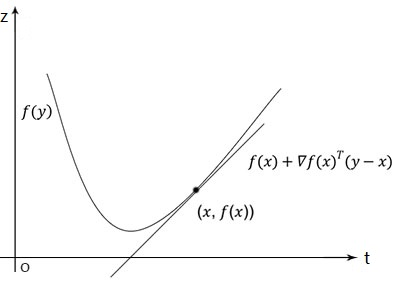
\includegraphics[height=3cm,width=6cm]{修改_第二章图2-2}
    \end{figure}
   
\end{frame}
%----------------------------------------------
\begin{frame}
	\frametitle{二阶条件}
	$f$ 是 \textbf{二阶可微的} 即 $\textbf{dom}\ f$ 是开的 ,且Hessian阵 $\nabla^{2} f(x) \in \mathbf{S}^{n}$,
	\begin{equation}
		\nabla^{2} f(x)_{i j}=\frac{\partial^{2} f(x)}{\partial x_{i} \partial x_{j}}, \quad i, j=1, \ldots, n
	\end{equation}
    存在于每个点 $x \in \textbf{dom}\ f$\\

    \begin{mytheorem}[二阶条件**] 在凸有效域上的二次可微函数 $f$ 
    \begin{itemize}
    	\item $f$ 是凸的,当且仅当
    	\begin{equation}
    		\nabla^{2} f(x) \succeq 0 \quad \text { 任意 } x \in \textbf{dom}\ f
    	\end{equation}\\
    	\bigskip
    	\item 如果 $\nabla^{2} f(x) \succ 0$ , $x \in \textbf{dom}\ f$,那么 $f$ 是严格凸的
    \end{itemize}
    \end{mytheorem}

\end{frame}
%----------------------------------------------
\begin{frame}
	\frametitle{示例}
\begin{itemize}[<+->]
  \item \textbf{二次函数** } $f(x)=(1 / 2) x^{T} P x+q^{T} x+r\left(\right.$  $\left.P \in \mathbf{S}^{n}\right)$
	\begin{equation}
		\nabla f(x)=P x+q, \quad \nabla^{2} f(x)=P
	\end{equation}
    是凸函数, 当$P \succeq 0$时

  \item  \textbf{最小二乘**} $f(x)=\|A x-b\|_{2}^{2}$
    \begin{equation}
    	\nabla f(x)=2 A^{T}(A x-b), \quad \nabla^{2} f(x)=2 A^{T} A
    \end{equation}
    是凸函数 $($ 对于任意 $A)$


 \item \textbf{quadratic-over-linear}
    \begin{columns}
    	\column{0.4\textwidth}
    	$f(x, y)=x^{2} / y$
    	\begin{equation}
    		\nabla^{2} f(x, y)=\frac{2}{y^{3}}\left[\begin{array}{c}
                 y \\
                 -x
                 \end{array}\right]
                 \left[\begin{array}{c}
                 y \\
                 -x
                 \end{array}\right]^{T} \succeq 0
    	\end{equation}
        是凸函数,当$y>0$时
    	\column{0.5\textwidth}
    	\begin{figure}
    		\centering
    		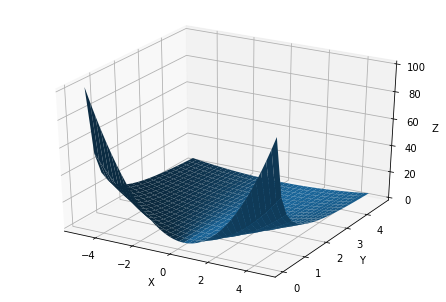
\includegraphics[width=0.9\columnwidth]{修改2-3}
    	\end{figure}
    \end{columns}

\end{itemize}
	
\end{frame}
%-------------------------------------
\begin{frame}
	\frametitle{示例}

\begin{itemize}[<+->]
  \item \textbf{对数和表达式**} $f(x)=\log \sum_{k=1}^{n} \exp x_{k}$ 是凸函数
	\begin{equation}
		\nabla^{2} f(x)=\frac{1}{\mathbf{1}^{T} z} \text{diag}(z)-\frac{1}{\left(\mathbf{1}^{T} z\right)^{2}} z z^{T} \quad\left(z_{k}=\exp x_{k}\right)
	\end{equation}\\
	\bigskip
    为了展示 $\nabla^{2} f(x) \succeq 0$, 我们必须证明对于所有$v$ ,$v^{T} \nabla^{2} f(x) v \geq 0$  :
    \begin{equation}
    	v^{T} \nabla^{2} f(x) v=\frac{\left(\sum_{k} z_{k} v_{k}^{2}\right)\left(\sum_{k} z_{k}\right)-\left(\sum_{k} v_{k} z_{k}\right)^{2}}{\left(\sum_{k} z_{k}\right)^{2}} \geq 0
    \end{equation}\\
    \bigskip
    因为$\left(\sum_{k} v_{k} z_{k}\right)^{2} \leq\left(\sum_{k} z_{k} v_{k}^{2}\right)\left(\sum_{k} z_{k}\right)$ (来自柯西-施瓦兹不等式)\\
    \end{itemize}
\end{frame}
\begin{frame}
	\frametitle{示例}
	\begin{itemize}[<+->]
		\item $f(x)=\log (e^{x}+e^{y})$的图像
	

    \begin{figure}
    	\centering
    	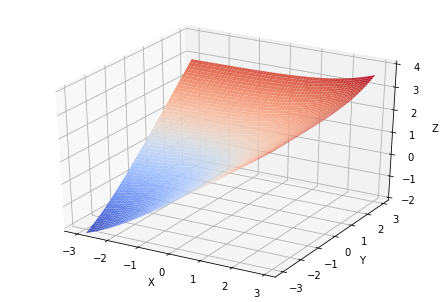
\includegraphics[width=0.6\columnwidth]{修改2-4}
    \end{figure}

   \item \textbf{几何平均** } $f(x)=\left(\prod_{k=1}^{n} x_{k}\right)^{1 / n}$ 在 $\mathbb{R}_{++}^{n}$ 上是凹的\\
    (与对数和表达式的证明相似)
\end{itemize}
	


\end{frame}
%-------------------------------------------
\begin{frame}
	\frametitle{上图(Epigraph)}
	
函数 $f的: \mathbb{R}^{n} \rightarrow \mathbb{R}$ 的\textbf{epigraph} 定义为:
    \begin{equation}
    	\textbf{ epi } f=\left\{(x, t) \in \mathbb{R}^{n+1} \mid x \in \textbf{dom}\ f, f(x) \leq t\right\}
    \end{equation}
     \begin{figure}
    	\centering
    	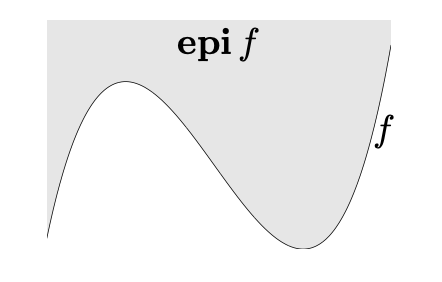
\includegraphics[width=0.3\columnwidth]{Ch3-Epigraph-and-sublevel-set}
    \end{figure}
    


\begin{mytheorem}[凸函数的Epigraph**]
  $f$ 是凸函数,当且仅当\textbf{epi} $f$ 是一个凸集.
\end{mytheorem}

\begin{figure}
	\centering
	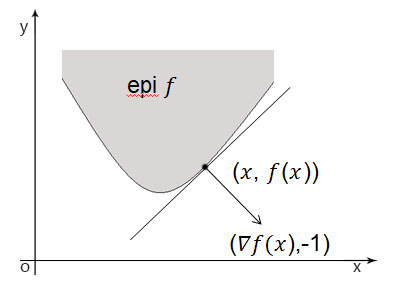
\includegraphics[width=0.3\columnwidth]{修改_第二章图2-6}
\end{figure}
\quad \quad  \quad \quad  \quad  \quad \quad \quad \quad \quad \quad 上图的一个支撑超平面

    %\begin{figure}
%    	\centering
%    	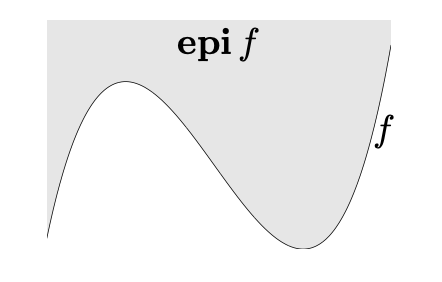
\includegraphics[height=4cm,width=6cm]{Ch3-Epigraph-and-sublevel-set}
%    \end{figure}

\end{frame}


\begin{frame}
	\frametitle{下水平集}
	$f$ 的\textbf{下水平集}- $\alpha$ :$ \mathbb{R}^{n} \rightarrow \mathbb{R}:$
	\begin{equation}
		C_{\alpha}=\{x \in \textbf{dom}\ f \mid f(x) \leq \alpha\}
	\end{equation}
    \textrm{凸函数的下水平集是凸的 (反之,逆命题未必成立)}

\end{frame}
%-------------------------------------------
\begin{frame}
	\frametitle{Jensen不等式}

\begin{itemize}[<+->]
  \item \textbf{基本不等式:} 如果 $f$ 是凸函数, 那么对于$0 \leq \theta \leq 1$有
	\begin{equation}
		f(\theta x+(1-\theta) y) \leq \theta f(x)+(1-\theta) f(y)
	\end{equation}

\item
	\textbf{扩展:}如果$f$ 是凸函数, 那么
	\begin{equation}
		f(\mathbf{E} z) \leq \mathbf{E} f(z)
	\end{equation}
    对于任何随机变量 $z$\\

  \item 基本不等式是离散分布的特例
    \begin{equation}
    	\textbf{prob}(z=x)=\theta, \quad \textbf{prob}(z=y)=1-\theta
    \end{equation}
\end{itemize}
	
\end{frame}
%===================================================
\section{保持凸性的运算}

\begin{frame}
\mytitle{\secno \secname}

	
\normaltitle{检验函数凸性的实用方法}

\begin{enumerate}
  \item 验证定义(通常通过限制到直线来简化)\\
\item 对于两次可微函数,验证 $\nabla^{2} f(x) \succeq 0$\\
\item 证明 $f$ 是通过保持凸性的运算从简单凸函数获得的\\

    \begin{itemize}
    	\item 非负加权求和
    	\item 复合仿射函数
    	\item 逐点最大和逐点上确界
    	\item 复合运算
    	\item 最小化
    	\item 透视函数(Perspective function)
    \end{itemize}
\end{enumerate}

\end{frame}
%---------------------------------------------
\begin{frame}
	\frametitle{正加权和 $\&$ 复合仿射函数}

\begin{itemize}
  \item \textbf{非负倍数:} 如果 $f$ 是凸函数,$\alpha f$ 是凸函数, $\alpha \geq 0$\\

	\item \textbf{求和:} 如果 $f_{1}, f_{2}$ 都是凸函数,$f_{1}+f_{2}$ 是凸函数 (扩展到无限和、积分)\\
	
\item	\textbf{复合仿射函数:}  如果 $f$ 是凸函数,$f(A x+b)$ 是凸函数\\
	
\end{itemize}
	
\onslide<2->{
	\textbf{示例}

	\begin{itemize}
		\item \hint{线性不等式的对数和}
		\begin{equation}
			f(x)=-\sum_{i=1}^{m} \log \left(b_{i}-a_{i}^{T} x\right), \quad \textbf { dom } f=\left\{x \mid a_{i}^{T} x<b_{i}, i=1, \ldots, m\right\}
		\end{equation}
		\item \hint{(任意) 仿射函数的范数: $f(x)=\|A x+b\|$}
	\end{itemize}
}
\end{frame}
%----------------------------------------
\begin{frame}
	\frametitle{逐点最大值}
\begin{mytheorem}
  如果 $f_{1}, \ldots, f_{m}$ 都是凸函数, 则 $f(x)=\max \left\{f_{1}(x), \ldots, f_{m}(x)\right\}$ 是凸函数.	
\end{mytheorem}
	


\onslide<2->{
	\textbf{示例:}
}

	\begin{itemize}%[<+->]
		\item<2-> 分段线性函数: $f(x)=\max _{i=1, \ldots, m}\left(a_{i}^{T} x+b_{i}\right)$ 是凸函数
		\item<3-> $x$的 $r$ 个最大分量之和 $x \in \mathbb{R}^{n}$ :
		\begin{equation}
			f(x)=x_{[1]}+x_{[2]}+\cdots+x_{[r]}
		\end{equation}
		是凸函数 $\left(x_{[i]}\right.$ 是$\left.x\right)$第 $i$ 个最大分量 

		 \item<4-> 证明:
       \begin{equation}
	   f(x)=\max \left\{x_{i_{1}}+x_{i_{2}}+\cdots+x_{i_{r}} \mid 1 \leq i_{1}<i_{2}<\cdots<i_{r} \leq n\right\}
       \end{equation}
	\end{itemize}


\end{frame}
%--------------------------------------------------
\begin{frame}
	\frametitle{逐点上确界{$\leftarrow$ 逐点最大值}}
\begin{mytheorem}
	如果 $f(x, y)$ 关于$x$是凸的,对任意$y \in \mathcal{A},$ 则
	\begin{equation}
		g(x)=\sup _{y \in \mathcal{A}} f(x, y).
	\end{equation}
    也是凸函数
\end{mytheorem}

 \tinyhint{证. $f_i(\theta x_1 +(1-\theta)x_2)\leq f(x_1)+ (1-\theta)f(x_2)$, $i=1,\cdots,m$, $\theta\in (0,1)$}
 
\onslide<2->{
	\textbf{示例}
}
    \begin{itemize}
    	\item<2-> 集合的支持函数 $C: S_{C}(x)=\sup _{y \in C} y^{T} x$ 是凸的
    	\item<3-> 到集合中最远点的距离 $C$ \footnotehint{(选讲)} :
    	\begin{equation}
    		f(x)=\sup _{y \in C}\|x-y\|
    	\end{equation}
    	\item<4-> 对称矩阵的最大特征值: for $X \in \mathbf{S}^{n}$,
    	\begin{equation}
    		\lambda_{\max }(X)=\sup _{\|y\|_{2}=1} y^{T} X y
    	\end{equation}
    \end{itemize}
\end{frame}
%--------------------------------------------
\begin{frame}
	\frametitle{标量函数组合}
\begin{mytheorem}
	 给定函数$g: \mathbb{R}^{n} \rightarrow \mathbb{R}$ 和 $h: \mathbb{R} \rightarrow \mathbb{R}:$
	\begin{equation}
		f(x)=h(g(x))
	\end{equation}
    $f$ 是凸函数 如果
    \begin{itemize}
    	\item[-] $g$ 是凸函数, $h$ 是凸函数, $\tilde{h}$ 非减;
    	\item[-] $g$ 是凹函数, $h$ 是凸函数, $\tilde{h}$ 非减.
    \end{itemize}
\end{mytheorem}

	\begin{itemize}
		\item<2-> 证明 (当 $n=1$, 函数 $g, h$可微)
		\begin{equation}
			f^{\prime \prime}(x)=h^{\prime \prime}(g(x)) g^{\prime}(x)^{2}+h^{\prime}(g(x)) g^{\prime \prime}(x)
		\end{equation}
		\item<3-> 注意:单调性必须适用于扩展值扩展 $\tilde{h}$
	\end{itemize}
	
\onslide<4->{
	\textbf{示例:}
}
	\begin{itemize}
		\item<4-> 如果 $g$ 是凸函数,$\exp g(x)$ 是凸函数
		\item<5-> 如果 $g$ 是凹函数且为正,$1 / g(x)$ 是凸函数
	\end{itemize}
\end{frame}


%-------------------------------------------
\begin{frame}
	\frametitle{向量组合}
	给定函数 $g: \mathbb{R}^{n} \rightarrow \mathbb{R}^{k}$ 和 $h: \mathbb{R}^{k} \rightarrow \mathbb{R}$ :
	\begin{equation}
		f(x)=h(g(x))=h\left(g_{1}(x), g_{2}(x), \ldots, g_{k}(x)\right)
	\end{equation}\\
	$f$ 是凸函数如果
	\begin{itemize}
		\item[-] $g_{i}$ 是凸函数, $h$ 是凸函数, $\tilde{h}$ 在每个参数中非减
		\item[-] $g_{i}$ 是凹函数, $h$ 是凸函数, $\tilde{h}$ 在每个参数中非减

	\end{itemize}
	\bigskip
    证明 $($ 当 $n=1,$ 函数$g, h$可微)
    \begin{equation}
    	f^{\prime \prime}(x)=g^{\prime}(x)^{T} \nabla^{2} h(g(x)) g^{\prime}(x)+\nabla h(g(x))^{T} g^{\prime \prime}(x)
    \end{equation}\\
    \bigskip
    \textbf{示例}\\
    \begin{itemize}
    	\item 如果 $g_{i}$ 是凹函数且为正,则$\sum_{i=1}^{m} \log g_{i}(x)$ 是凹函数
    	\item 如果$g_{i}$ 是凸函数,则$\log \sum_{i=1}^{m} \exp g_{i}(x)$ 是凸函数
    \end{itemize}
\end{frame}
%--------------------------------------------
\begin{frame}
	\frametitle{最小化}
	如果 $f(x, y)$ 在$(x, y)$上是凸函数  ,且 $C$ 是一个凸集, 则
	\begin{equation}
		g(x)=\inf _{y \in C} f(x, y)
	\end{equation}
	是凸函数\\
	\bigskip
	\textbf{示例:}
	\begin{itemize}
		\item $f(x, y)=x^{T} A x+2 x^{T} B y+y^{T} C y$ 
		\begin{equation}
			\left[\begin{array}{cc}
            A & B \\
            B^{T} & C
        \end{array}\right] \succeq 0, \quad C \succ 0
		\end{equation}
		在 $y$上最小化,令 $g(x)=\inf _{y} f(x, y)=x^{T}\left(A-B C^{-1} B^{T}\right) x$
        $g$ 是凸函数, 因此Schur补 $A-B C^{-1} B^{T} \succeq 0$
		\item 到集合的距离: 如果 $S$ 是凸函数,则$\textbf{dist}(x, S)=\inf _{y \in S}\|x-y\|$ 是凸函数
	\end{itemize}
\end{frame}
%------------------------------------
\begin{frame}
	\frametitle{透视函数(Perspective function)}

\begin{mydefinition}
	函数的$f: \mathbb{R}^{n} \rightarrow \mathbb{R}$ 的 \textbf{透视}  是函数$g: \mathbb{R}^{n} \times \mathbb{R} \rightarrow \mathbb{R}$
	\begin{equation}
		g(x, t)=t f(x / t), \quad \textbf{dom} g=\{(x, t) \mid x / t \in \textbf{dom} f, t>0\}
	\end{equation}
	
\end{mydefinition}


\onslide<2->{
命题: 如果 $f$是凸函数,则 $g$ 是凸函数

}

\onslide<3->{	
	\begin{itemize}
		\item $f(x)=x^{T} x$ 是凸函数; 那么 $g(x, t)=x^{T} x / t$ 是凸函数当 $t>0$时
		\item 负对数函数 $f(x)=-\log x$ 是凸的; 那么相对熵 $g(x, t)=t \log t-t \log x$ 在 $\mathbb{R}_{++}^{2}$上也是凸的
		\item 如果 $f$ 是凸函数, 那么
		\begin{equation}
			g(x)=\left(c^{T} x+d\right) f\left((A x+b) /\left(c^{T} x+d\right)\right)
		\end{equation}
		也是凸函数 ,其中$\left\{x \mid c^{T} x+d>0,(A x+b) /\left(c^{T} x+d\right) \in \textbf{dom} f\right\}$
	\end{itemize}
}

\end{frame}

%===================================================
\section{共轭函数}
\begin{frame}
%	\frametitle{共轭函数}
\mytitle{\secno \secname}

\bigskip

\begin{mydefinition}
	 函数 $f$ 的\textbf{共轭函数} 为
	\begin{equation}
		f^{*}(y)=\sup _{x \in \textbf{dom} f}\left(y^{T} x-f(x)\right)
	\end{equation}
\end{mydefinition}

%	\begin{figure}
%		\centering
%		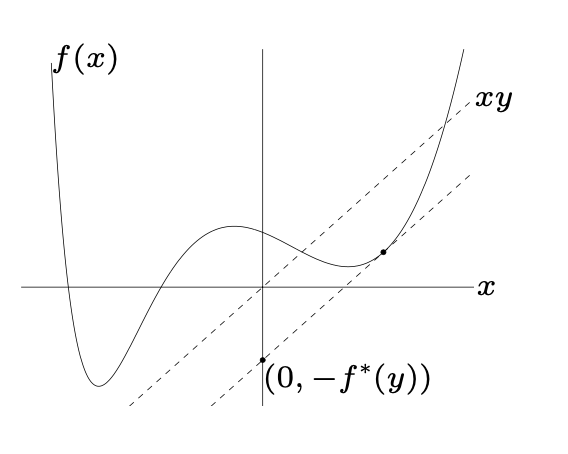
\includegraphics[height=4cm,width=6cm]{Ch3-The-conjugate-function}
%	\end{figure}

\onslide<2->{
	\begin{itemize}
		\item $f^*$ 是凸的 (即使 $f$ 不是凸的)
		\item 将在第5章中运用
	\end{itemize}
}

\end{frame}
%------------------------------------
\begin{frame}
	\frametitle{共轭函数}
	\textbf{示例:}
	
	\begin{itemize}[<+->]
		\item 负对数函数: $f(x)=-\log x$
		\begin{equation}
			\begin{aligned}
            f^{*}(y) &=\sup _{x>0}(x y+\log x) \\
            &=\left\{\begin{array}{ll}
            -1-\log (-y) & y<0 \\
            \infty & \text { 其他 }
            \end{array}\right.
            \end{aligned}
		\end{equation}
		
		\item 严格凸二次型: $f(x)=(1 / 2) x^{T} Q x$ , $Q \in \mathbf{S}_{++}^{n}$
		\begin{equation}
			\begin{aligned}
            f^{*}(y) &=\sup _{x}\left(y^{T} x-(1 / 2) x^{T} Q x\right) \\
            &=\frac{1}{2} y^{T} Q^{-1} y
            \end{aligned}
		\end{equation}
	\end{itemize}

\end{frame}

\section{次梯度与次微分}

\begin{frame}
	\frametitle{次梯度}	
	\normaltitle{定义}
	$f: \mathbb{R}^{n} \rightarrow \mathbb{R}$ 是凸函数,如果$x^{*}$满足
	\begin{equation}
		f(z) \geq f(x)+ \langle x^{*},z-x\rangle  \qquad\forall z \in \mathbf{R}^{n}
	\end{equation}
	则称向量$x^{*}$为凸函数 $f$在点$x$处的次梯度
	\begin{itemize}[<+->]
		\item 当 $f$在$x$处有限时,它有明显的几何意义:\\仿射函数$h(z)=f(x)+(x^{*})^{T}(z-x)$的图形是凸集$epif$在点$(x,f(x))$处的非垂直的支撑超平面
	\end{itemize}
	\begin{mytheorem}
	设$S$是一个开凸集,函数$f:S \rightarrow R$是凸函数。当且仅当对所有的$\omega \in \mathbf{S}$,存在$z$满足
		\begin{equation}
			f(\mu) \geq f(\omega)+ \langle\mu-\omega,z\rangle \qquad\forall \mu \in \mathbf{S}
		\end{equation}
	\end{mytheorem}
	依据此引理,对于恰当凸函数,$f(\omega)$为最小值的充要条件是$0 \in \partial f(\omega)$,即零向量是$f$在$\omega$处的次梯度。

\end{frame}
\begin{frame}
	\frametitle{次微分}	
	\normaltitle{定义}
	在$x$的所有次梯度的集合称为 $f$在 $x$的次微分,记为$\partial f(x)$
	\begin{itemize}[<+->]
		\item $\partial f(x)$可以是空集,也可以只由一个向量组成,如果 不为空,则称 $f$在 $x$处次可微。如果f在 $\omega$处是可微的,那么  $\partial f(\omega)$只包含一个元素,即 $f$在$\omega$ 处的梯度。
		\item 凸函数的次微分总是非空,因为凸函数总是存在次梯度
	\end{itemize}
	
\end{frame}
\section{对偶}
\begin{frame}
	\frametitle{对偶关系}	
	\begin{mytheorem}对于任意正常凸函数$f$ 和任意向量$x$,关于向量 $x^{*}$的下列四个条件彼此等价: \\
		\begin{itemize}[<+->]
			\item $x^{*} \in\partial f(x)$
			\item $z^{T}x^{*}-f(z)$在 $z=x$处取到关于 $z$的上界
			\item $f(x)+f^{*}(x^{*})\leq x^{T}x^{*}$
			\item $f(x)+f^{*}(x^{*})= x^{T}x^{*}$\\
			如果$(clf)(x)=f(x)$ ,这个相互等价条件的列表中还可以增加以下三个条件:
			\item $x \in \partial f^{*}(x^{*})$
			\item  $x^{T}z^{*}-f^{*}(z^{*})$在 $z^{*}=x^{*}$处取到关于 $z^{*}$中的上界
			\item $x^{*} \in\partial (clf)(x)$
		\end{itemize}	
	\end{mytheorem}
	
\end{frame}

%---------------------------------------------
%\begin{frame}
%	\frametitle{Properties of log-concave functions}
%	\begin{itemize}
%		\item twice differentiable $f$ with convex domain is log-concave if and only if
%		\begin{equation}
%			f(x) \nabla^{2} f(x) \preceq \nabla f(x) \nabla f(x)^{T}
%		\end{equation}
%		for all $x \in \textbf{dom} f$\\
%		\bigskip
%		\item product of log-concave functions is log-concave\\
%		\bigskip
%		\item sum of log-concave functions is not always log-concave\\
%		\bigskip
%		\item integration: if $f: \mathbb{R}^{n} \times \mathbb{R}^{m} \rightarrow \mathbb{R}$ is log-concave, then
%		\begin{equation}
%			g(x)=\int f(x, y) d y
%		\end{equation}
%		is log-concave (not easy to show)
%	\end{itemize}
%\end{frame}
%------------------------------------------
%\begin{frame}
%	\frametitle{Properties of log-concave functions}
%	\textbf{consequences of integration property}
%	\begin{itemize}
%		\item convolution $f * g$ of log-concave functions $f, g$ is log-concave
%		\begin{equation}
%			(f * g)(x)=\int f(x-y) g(y) d y
%		\end{equation}\\
%		\bigskip
%		\item if $C \subseteq \mathbb{R}^{n}$ convex and $y$ is a random variable with log-concave pdf then
%		\begin{equation}
%			f(x)=\textbf{prob}(x+y \in C)
%		\end{equation}
%		is log-concave\\
%		\bigskip
%		proof: write $f(x)$ as integral of product of log-concave functions
%		\begin{equation}
%			f(x)=\int g(x+y) p(y) d y, \quad %g(u)=\left\{\begin{array}{ll}
     %           1 & u \in C \\
      %          0 & u \notin C,
       %         \end{array}\right.
		%\end{equation}
		%$p$ is pdf of $y$
	%\end{itemize}
%\end{frame}
%-------------------------------------------
%\begin{frame}
%	\frametitle{Properties of log-concave functions}
%	\textbf{example: yield function}
%	\begin{equation}
%		Y(x)=\textbf{prob}(x+w \in S)
%	\end{equation}\\
%	\begin{itemize}
%		\item $x \in \mathbb{R}^{n}:$ nominal parameter values for product
%		\item $w \in \mathbb{R}^{n}:$ random variations of parameters in manufactured product
%		\item $S:$ set of acceptable values
%	\end{itemize}
%	\bigskip
%	\bigskip
%	if $S$ is convex and $w$ has a log-concave pdf, then
%	\begin{itemize}
%		\item $Y$ is log-concave
%		\item yield regions $\{x \mid Y(x) \geq \alpha\}$ are convex
%	\end{itemize}
%\end{frame}
%===================================================
%\section{convexity with respect to generalized inequalities}
%\begin{frame}
%	\frametitle{Convexity with respect to generalized inequalities}
%	$f: \mathbb{R}^{n} \rightarrow \mathbb{R}^{m}$ is $K$ -convex if $\textbf{dom}\ f$ is convex and
%	\begin{equation}
%		f(\theta x+(1-\theta) y) \preceq_{K} \theta f(x)+(1-\theta) f(y)
%	\end{equation}
%	for $x, y \in \textbf{dom}\ f, 0 \leq \theta \leq 1$\\
%	\bigskip
%	\textbf{example} $f: \mathbf{S}^{m} \rightarrow \mathbf{S}^{m}, f(X)=X^{2}$ is $\mathbf{S}_{+}^{m}$ -convex\\
%	\bigskip
%	proof: for fixed $z \in \mathbb{R}^{m}, z^{T} X^{2} z=\|X z\|_{2}^{2}$ is convex in $X,$ i.e.,
%	\begin{equation}
%		z^{T}(\theta X+(1-\theta) Y)^{2} z \leq \theta z^{T} X^{2} z+(1-\theta) z^{T} Y^{2} z
%	\end{equation}
%	for $X, Y \in \mathbf{S}^{m}, 0 \leq \theta \leq 1$\\
%	\bigskip
%	therefore $(\theta X+(1-\theta) Y)^{2} \preceq \theta X^{2}+(1-\theta) Y^{2}$
%\end{frame}
\begin{frame}
	\frametitle{总结:凸函数.}
	
	\begin{itemize}
		\item 定义
		
		\begin{itemize}
			\item 定义\,1. \mystar $f$ 是凸函数:
			$f(\theta x + (1-\theta)y) \leq \theta f(x) + (1-\theta) f(y)$, $\forall x,y \in \dom f$, $\theta \in (0,1)$.
			
			\footnotehint{严格凸}
			
			\item  定义\,2.\mystar $f$ 是凸函数当且仅当$\mathbf{epi}\,f$ 是一个凸集.
			
			\item   Jensen不等式.
			
			$f$ 是凸函数 $\Rightarrow$ $f(\bbe \bfX) \leq \bbe f(\bfX)$
		\end{itemize}
		
	\end{itemize}

	\begin{itemize}
		\item 凸函数的示例 \mystar
		
		\begin{itemize}
			\item $\bbr$上的示例: $ax+b$, $e^{ax}$ ($a\in \bbr$),
			$x^\alpha$, $x>0$, $\alpha\geq 1$, $x\log x$, $- \log x$
			
			\item  $\bbr^n$上的示例: $\langle a,x\rangle +b$, $\|x\|_p$
			
			\item $\bbr^{m\times n}$的示例: $\trace(A^TX)+b$, $\|X\|_2 = \lambda_{\max}^{}(X_{}^T X)^{1/2}$
			\item 其他:
			
			凸集上的指示函数: $ I_C(x)$
		\end{itemize}
	\end{itemize}

	\begin{itemize}
		
		\item 性质
		
		\begin{itemize}
			\item 性质.\mystar 凸函数$f$对直线的限制:
			$g(t) = f(x+tv)$, $v\in \bbr^n$
			
			\smallhint{e.g. $f(X) = \log \textnormal{det}X$ 是凹函数 }
			
			
		\end{itemize}
	\end{itemize}

\end{frame}

\begin{frame}
\frametitle{总结:凸函数.}
\begin{itemize}
	\item 定理
	\begin{itemize}
		
		\item 定理  (一阶条件\doublestar)
		
		函数 $f\in \calc^1$ 是凸函数
		$\Leftrightarrow$ $f(y) \geq f(x) + \nabla f(x)^T (y-x)$, $
		\forall x,y \in \dom f$.
		
		
		\item 定理 (二阶条件\mystar)
		
		
		函数 $f\in \calc^2$ 是凸函数
		$\Leftrightarrow$ $ \nabla^2 f(x)\succeq 0$, $
		\forall x \in \dom f$.
		
		函数 $f\in \calc^2$ 是 \hint{严格凸的}
		$\Leftarrow$  $ \nabla^2 f(x)\succ 0$, $ \forall x \in \dom f$
	\end{itemize}
\end{itemize}

\begin{itemize}
	
	\item 凸函数的示例
	
	\begin{itemize}
		\item 二次函数:\doublestar $f(x) = \frac{1}{2} x^T Px + c^T x +r $, $P\succeq 0$
		
		\item 最小二乘:\doublestar $f(x) = \|Ax-b\|^2$
		
		
		\item 对数和表达式: $f(x) = \log \sum_{i=1}^n e^{x_i}$
		
	\end{itemize}
	
	
	\hint{其他示例 }
	
	\begin{itemize}
		
		\item 二次超线性函数: $f(x,y) = x^2/y$, $y>0$
		
		
		\item 几何平均: $f(x)= (\prod_{i=1}^n x_i)^{1/n}$, $x\in \bbr^n_{++}$
		
		\item 矩阵分数函数: $f:\bbr^n\times \bbf^n_{++} \rightarrow \bbr$,
		$f(x,Y) = x^{\top}Y^{-1}x $
		
	\end{itemize}
\end{itemize}

\end{frame}


\begin{frame}
\frametitle{总结:凸函数.}
\begin{itemize}

\item 保持凸性的运算

$f$, $f_1,\cdots, f_m$: 凸函数 $\Rightarrow$
以下均是凸的:

\begin{footnotesize}
	
	\begin{itemize}
		\item $\alpha f$, $\alpha >0$
		\item $f_1 + f_2$ $\rightarrow$ 无限求和
		\item $f(Ax+b)$
		
		\footnotehint{e.g., $f(x) = - \sum_{i=1}^m \log (b_i-a_i^T x)$,
			$a_i^Tx<b$, $i=1,\cdots,m$.
		}
		\item 逐点最大值: $f(x) = \max\{f_1(x),\cdots, f_m(x)\}$
		
		\footnotehint{e.g., $x$上的$r$个最大分量求和 $\in\bbr^n$ \doublestar}
		
		\item 逐点上确界:
		$
		g(x)\defeq \sup_{y\in \cala}^{} f(x,y)
		$
		
		$f(x,y)$ 是关于 $x$凸的对每个 $y\in \cala$,
		
		\footnotehint{e.g.,  支持函数,\doublestar $\lambda_{\max}(X)$} \doublestar
		
		\item 最小化: $g(x) = \inf_{y\in C} f(x,y)$
		
		\hint{$f(x,y)$: 在$(x,y)$上凸的}, $C$:凸集
		
		\footnotehint{e.g.,\doublestar $\dist(x,S)$}
		
		\item 复合运算:\mystar  $h(g(x))$, $g$: 凸的, $h$: 凸的, 上升的
	\end{itemize}
	
\end{footnotesize}
\end{itemize}

\end{frame}

\begin{frame}
\frametitle{总结:凸函数.}
\begin{itemize}
\item 共轭函数

\begin{itemize}
	\item 定义.\mystar $f^*(x^*) = \sup_{x} (\langle x^*,x\rangle - f(x))$
	
	\item   e.g., 计算以下各项的共轭函数:\doublestar
	
	$f(x) =-\log x$,
	
	$f(x) = \frac{1}{2}x^{T}Qx$, $Q\in \bfS^n_{++}$,
	
	$f(x) = I_C(x)$,
	
	$f(x) = \frac{1}{2}\|x\|^2$, $\|\cdot\|$ 是一个范数,
	%$\rightarrow$ $f^*=?$
	
\end{itemize}
\end{itemize}

\begin{itemize}
\item 凸函数的次微分

\begin{itemize}
	\item 定义.\mystar $\partial f(x) =  \{ x^* | f(y) \geq f(x) + \langle x^*,y-x\rangle , \forall y \}$
	
	\item   e.g.,\doublestar $f(x) =\|x\|_1$,
	$\rightarrow$ $\partial f(x)=$ ?
	
\end{itemize}
\end{itemize}

\begin{itemize}
\item 对偶
\begin{itemize}
	\item 定理:四个等价条件
\end{itemize}
\end{itemize}

\end{frame}


\begin{frame}
\frametitle{总结:凸函数.}
\begin{itemize}
\item 凸集和凸函数

\medskip
\begin{footnotesize}
\begin{tabular}{ll}
	\toprule
	凸集 & 凸函数 \\
	\midrule
	$\textnormal{epi}f $ 凸函数 & $f$ 凸函数 \\  \midrule
	部分和 & \\
	\footnotesize{ $\left\{t_1+t_2 |\, (x,t_1) \in \epi f_1, \ (x,t_2)\in \epi f_2\right\}$ }  &     $f = f_1 + f_2$ \\  \midrule
	$\epi f = \cala \,\epi f_1$ $\cala: (x,\frac{t}{\alpha}) \mapsto (x,t)$   &     $f = \alpha f_1$ \\ \midrule
	$\epi f = \textnormal{prog}_x \epi g$   & $f(x) = \inf_{y\in C} g(x,y)$\\ \midrule
	$\epi f =  \epi f_1 \cap \epi f_2$   & $f(x) =  \max\{f_1(x),f_2(x)\}$\\ \midrule
	$\epi f = \cala\, \epi g $ $\cala: (x, {\alpha}) \mapsto (x,h(\alpha))$  &       $ f(x)  = h(g(x))$ \\

$\epi g = \cala^{-1} \epi f$  & 透视函数 \\
		$\cala:  \bbr^{n+1+1} \rightarrow \bbr^{n+1}$  &  \quad $g(x,t) = t   f(\frac{x}{t}), \ t>0$    \\
		$\cala(u,v,w) = (u,w)/v   $    & \\ \midrule
		\multirow{2}{*}{ $\epi f =  \epi f_1 + \epi f_2$ }  & 卷积下确界: $f = f_1 \square  f_2 $ \\
		& \quad $f(x) = \inf_{x_1 + x_2 = x}  f_1(x_1) +f_2(x_2)  $ \\ \midrule
		\multirow{2}{*}{ $\epi f =  \lambda \epi f_1  $ }   & 右乘法 \\
		& $(f\lambda)(x) =  \lambda\cdot f(\lambda^{-1}x)$   \\

	\bottomrule
\end{tabular}
\end{footnotesize}

\end{itemize}
\end{frame}





